\section{Categorizing Verified Programming Tools}\label{S:categories}

I propose 3 axes along which to classify the tools used to verify programs.
These are
\begin{enumerate}
    \item the type of interaction;
    \item the type of proof logic; and
    \item the type of supported programming languages.
\end{enumerate}

I examine each in turn in Sections~\ref{S:t_interaction},~\ref{S:t_logic},
and~\ref{S:t_pl}.

One might also include the logic of the underlying verifier, especially in cases
where it differs from the proof logic. I choose not to include the verifier's
logic because in the cases I have studied they are the same (\eg, a Coq program
proven in Coq~\cite{Coq}), one is encoded in the other (\eg, a
Dafny~\cite{leino2010dafny} program proven by translation to
Boogie~\cite{Barnett_2006,leino2008this}), or one is not relevant to the other
(\eg, proofs in Iris's logic~\cite{Jung_2018b} use Iris's proof rules, while
Iris is built on Coq). The encapsulation provided by many verifiers obviates a
need to consider their underlying logics. Except in the case of a leaky
abstraction~\cite{Spolsky_2002}, wherein the underlying verifier's logic leaks
out to the logic of the proof, the programmer tasked with writing the proof is
concerned with the proof-logic and the proof to be written. The
programmer interested in building a programming language for verified languages
should certainly study verification logic, in addition to verification logics
like \gls{smt} or \gls{coc} and the architectures of such verifiers (\eg, for
\gls{smt}, the original~\cite{Davis_1960,Davis_1962} or the newer
handbook~\cite{biere2009handbook}).

\subsection{Type of Interaction}\label{S:t_interaction}

In the context of a verified programming tool, ``interaction'' means that
between the programmer and the verifier: what is necessary to formulate proofs?
Borrowing the terminology of~\cite[\S 2]{Nelson_2019}, I dissect this axis into
3 major types of interaction.
\begin{description}
    \item[Interactive tools.] The programmer manually constructs the proof by
        manipulating facets of the tool, such as by invoking tactics, to
        progress towards a specified proof goal. Such tools may provide
        automation or proof-search mechanisms.
    \item[Auto-active tools.] The programmer and the tool share the burden of
        constructing a proof: the tool is capable of some automatic reasoning,
        but requires the programmer to manually fill in the gaps.
    \item[Automatic tools.] Sometimes called ``push-button'' tools. The
        programmer invokes the tool, which might find a proof, fail to find a
        proof, or produce a counter-example.
\end{description}

For each type, the reference~\cite{Nelson_2019} provides further examples.

\subsubsection{Interactive verification}

This is the model employed by interactive theorem-provers and proof-assistants
such as Coq~\cite{Coq}, Isabelle~\cite{Isabelle}, and HOL~\cite{HOL}. The
programmer, having written programs and specifications, states theorems relating
them (or lemmata, corollaries, \etc, as the case may be). In order to prove the
statements, the programmer interacts directly with the verifier in a sort of
call-and-response. The verifier presents a goal: prove this statement. The
programmer can execute tactics to manipulate the goal, introduce quantified
variables and hypotheses, and otherwise make progress towards the proof of the
goal. The verifier represents the effect of these executions with another
response, \eg, prove this statement in this context. The programmer continues
this dialogue with the verifier, perhaps walking backwards and trying a
different approach or walking forwards through the steps of the proof, until the
verifier has been given a complete proof of all necessary goals.

\begin{figure}[ht]
\begin{coq_example}
Goal forall P: Prop, P -> P.
intros.
assumption.
Qed.
\end{coq_example}
    \caption{Proving a simple tautology in Coq.}\label{F:coq1}
\end{figure}

The example in \figurename~\ref{F:coq1} demonstrates one Coq proof of a
simple tautology through tactics. The \texttt{intros} tactic introduces
quantified variables for manipulation; \texttt{assumption} looks for a
hypothesis in the context that matches the goal.

Such verifiers may support automation in the sense of tactics that invoke other
tactics based on the goal or context; these can range from proof searches to
constraint solvers over linear integer arithmetic to manipulations necessary to
hide details of the underlying logical verifier.

\begin{figure}[ht]
\begin{coq_eval}
Require Import List.
Import ListNotations.
\end{coq_eval}
\begin{coq_example}
Goal In 5 [1;2;3;4;5].
simpl; right; right; right; right.
(* too manual, try again *) Undo.
repeat (try (left; reflexivity); right).
Qed.
\end{coq_example}
    \caption{Proving a tedious proof with automation in Coq.}\label{F:coq2}
\end{figure}

For example, the prove in \figurename~\ref{F:coq1} is completely finished by
tactics like \texttt{tauto} or \texttt{auto}. Advanced automation can be used to
show \(5 \in [1,2,3,4,5]\), where the \(\func{In}\) relation below is computed
as follows: \(\func{In}\) is false for any value and the empty list.
\(\func{In}\) is true if either the value is the head of the list or it is in
the tail of the list. Without automation, the proof consists of the
\texttt{right} tactic four times to get to the correct disjunct; only then can
we finish by selecting the \texttt{left} case and proving it (trivially, \(5 =
5\)). This is explicated in \figurename~\ref{F:coq2}.

\subsubsection{Auto-active verification}

The approach taken by verifiers like Dafny~\cite{leino2010dafny}. The programmer
annotates code both with specifications and proof hints, such as pre- or post-
conditions or loop invariants. The verifier translates the source into a
verification condition and uses a constraint solver to finish the verification.
Some verifiers, such as Dafny, permit annotations that nearly rise to the level
of proof texts like those of interactive verification, with composable theorems
and lemmata in addition to functional specifications and standard annotations.
While writing the proofs, though, the current state of the  goal and proof
context are often hidden or implicit, since the verifier translates the goal and
context for the constraint solver\footnote{The original goal and context are of
course visible in the original statement being proven.}. A call-and-response
effort is possible in such verifiers to complete a proof, but a major challenge
is to discover what the automatic part of the verifier cannot prove and actively
provide effective hints to make progress. One power of this type of verifier is
to free the programmer from all the details of the proof; the verifier often can
handle simple statements on its own, while more complex statements can be proven
with only a few well-directed hints. On the other hand, discovering which hints
to use is like a game of ``20 Questions''\footnote{The programmer asks ``Would
you be able to make progress on the proof if I could convince you of \(P\)?''
Based on the verifier's response, which is essentially ``yes'' or ``no'', a
sub-proof of \(P\) is given through hints or not, and the game continues. The
summer course in~\cite{Kapritsos_2020} provides a detailed look at this style of
proof in Dafny.}, and the resulting proofs can be difficult to read.

\begin{figure}[ht]
\begin{verbatim}
predicate IsPrime(i:nat)
{
  i > 1 && (forall j | 1 < j < i :: i % j != 0)
}

method Main() {
  assert forall P :: P ==> P;
  assert 5 in [1,2,3,4,5];
  assert !IsPrime(0);
  assert !IsPrime(1);
  assert IsPrime(2);
  assert IsPrime(3);
  // counter example for the proof to work
  assert 6 % 3 == 0;
  assert !IsPrime(6);
}
\end{verbatim}
    \caption{Example auto-active proofs in Dafny. Responses are provided upon
    invoking the Dafny compiler.}\label{F:dafny_ex}
\end{figure}

The example proofs (\(\forall P, P \implies P\) and \(5\) is in a long list
containing \(5\)) in Dafny are completely automatically checked by the Dafny
compiler, as shown in \figurename~\ref{F:dafny_ex}. However, let's add the
\(\func{IsPrime}\) predicate. Dafny can automatically find proofs for the
primality of 0, 1, 2, and 3. At 6, however, Dafny doesn't know what to do, and
the hint \(6 \mod 3 = 0\) is necessary to prove 6 is not prime. Removing the
line causes a verification error; adding it gives Dafny enough to disprove the
disjunct. Discovering that this is the missing information is rather like taking
an educated guess.

\subsubsection{Automatic verification}

The approach taken by Rosette~\cite{Torlak_2013}. An automatic verifier
restricts the class of properties and programs that be verified in order to
fully automate the process. The essential limit is finitization: finite
specifications that can be implemented without unbounded loops allows symbolic
evaluation or execution to generate constraints that can be handed off to a
solver, much like in auto-active verification. The developer thus programs in
such a restricted verifier and pushes the ``verify button'', invoking the symbolic
evaluator and constraint solver. The limitations allow a greater degree of
automation than in the previous cases, leading to the descriptor ``push-button
verification''---no proof annotations are necessary. Such verifiers have been used
to build surprisingly sophisticated programs given the finitization requirement;
examples include the Yggdrasil file-system~\cite{Sigurbjarnarson_2016} and the
Hyperkernel \gls{os}~\cite{Nelson_2017}.

A related challenge is exponential path explosion: symbolic evaluation may have
to consider a rapidly growing number of symbolic paths while generating
constraints. Rosette takes steps to solve this via aggressive partial
evaluation~\cite{Torlak_2013,Torlak_2014}, lenient symbolic
execution~\cite{Chang_2018}, and
profiling~\cite{Bornholt_2018,Porncharoenwase_2020}. Also related, as in the
case of auto-active verification, is the challenge of communicating back to the
developer the meaning of the results in the program domain.

\subsection{Type of Proof Logic}\label{S:t_logic}

A full account of proof-logics for programs would be a long paper in its own
right and is out of scope for this report. Look no further than
\figurename~\ref{F:iris_complex} to see how complicated the topology of (a
subset of) proof-logics can be. Instead, I will mention a key proof-logic
(namely, Hoare logic) and some of its extensions. For another mention of
program- and proof- logics and their uses, see~\cite[\S 5]{Appel_2011}.

\begin{figure}
    \centering
    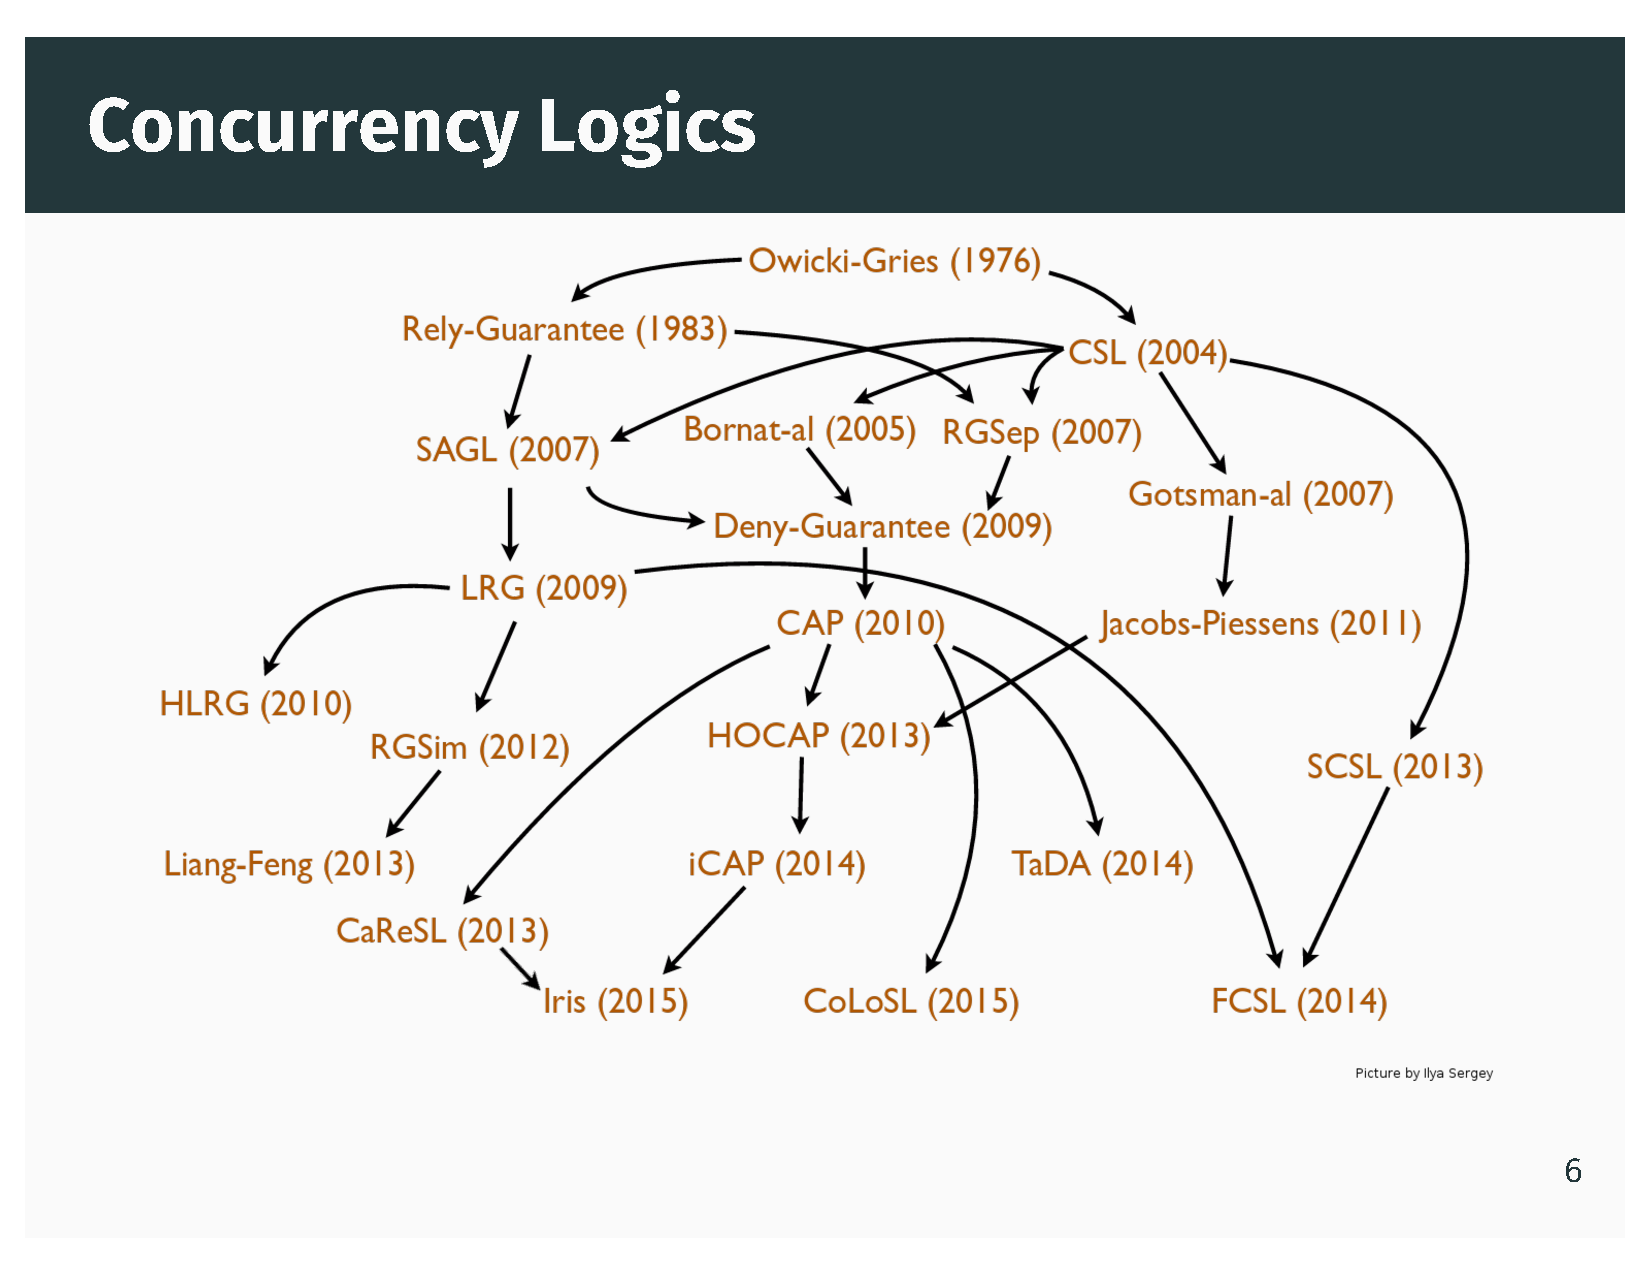
\includegraphics[width=\textwidth]{img/iris_2_0_concurrent_logics}
    \caption{A figure from a presentation on Iris~\cite{Jung_2016_slides}
    depicting the relationship of many concurrent separation logics developed
    specially for a system or proof. Iris notably attempts to distill these
    logics to their core, providing a verifier inside of which any of the
    individual logics may be derived.}\label{F:iris_complex}
\end{figure}

All proof-logics for programs combine a set of logic-rules with the semantics of
the program's language. In the simplest case, the programmer combines
``regular'' logic (in the sense of \gls{coc} or ZFC) with the semantics to write
proofs about program equivalences, termination, and transformations.
\emph{Software Foundations} shows it's possible to prove interesting
meta-theoretic\footnote{``meta'' because they are ``properties of the language
as a whole, rather than of particular programs''~\cite{Pierce:SF2}. It is also
possible to prove claims about specific programs this way, but, at least in some
verifiers, this becomes unwieldy.} claims about a language using these techniques
in their discussions about \emph{Simple Imperative Programs}~\cite{Pierce:SF1}
and \emph{Program Equivalence}~\cite{Pierce:SF2} and provides an introduction to
such proofs. Essentially, standard reasoning rules about logic formulae are
combined with the inference rules that define the semantics. An example is
provided in \figurename~\ref{F:Imp_ex}. I refer
to~\cite{Winskel_1993,Harper_2016} for introductions to program semantics.

\begin{figure}
    \centering
    \begin{mathpar}

        \inference[\iname{E-APlus}]{%
            \eval{\(e_1\)}{\sigma} = n_1 &
            \eval{\(e_2\)}{\sigma} = n_2
        }{\eval{\(e_1\) + \(e_2\)}{\sigma} = n_1 + n_2}

        \and

        \inference[\iname{E-Seq}]{%
            \comp{\(c_1\)}{\sigma_1} \DownTo \sigma_2 &
            \comp{\(c_2\)}{\sigma_2} \DownTo \sigma_3 &
        }{\comp{\(c_1\);\(c_2\)}{\sigma_1} \DownTo \sigma_3}

    \end{mathpar}
    \caption{Sample inference rules for \texttt{Imp}, a simple imperative
    language. \iname{E-APlus} shows how to add two arithmetic expressions, where
    \(\eval{e}{\sigma} = x\) means ``evaluation of \(e\) under a state
    \(\sigma\) produces \(x\).'' Similarly, \iname{E-Seq} shows how to sequence
    two statements \(c_1, c_2\), where \(\comp{c}{\sigma} \DownTo \sigma'\)
    means ``computing statement \(c\) in state \(\sigma\) produces the new state
    \(\sigma'\).''}\label{F:Imp_ex}
\end{figure}

\subsubsection{Hoare Logic}

When turning to program verification\footnote{Recall \citeauthor{EWD:EWD1036}'s
act of proving a program implements its specification.}, \emph{Software
Foundations} introduces Hoare logic. Hoare logic, with its many variations, is
the predominant proof-logic for program verification. Originating in
\citeyear{Hoare_1969} with \citeauthor{Hoare_1969}'s paper~\cite{Hoare_1969},
Hoare logic formalizes the notion of pre- and post-conditions with the
\emph{Hoare triple}, written

\begin{equation*}
    \{P\} C \{Q\},
\end{equation*}

to indicate that command \(C\) has pre-condition \(P\) and post-condition \(Q\),
both assertions (\eg, a claim about the current state). The triple states that,
if \(P\) is established, executing \(C\) establishes \(Q\) (or \(C\) diverges).
The programmer indicates that \(C\) diverges in a Hoare triple by choosing \(Q =
\bot\). Hoare logic permits reasoning about partial correctness; termination
must be proven separately\footnote{Various sources claim it is possible to give
rules for total correctness; the most complete rule I have seen involves
bounding loops with a well-founded order.}. The statement of the triple can thus
be written using notation from \figurename~\ref{F:Imp_ex}, and assuming \(P\)
and \(Q\) are functions from states to propositions

\begin{align*}
    \{P\} C \{Q\} \definedas \forall \sigma_1, \sigma_2 &: \comp{c}\sigma_1 \DownTo \sigma_2 &\text{if \(\mathtt{c}\) terminates} \\
    &\implies P \sigma_1 &\text{and if \(P \sigma_1\) holds} \\
    &\implies Q \sigma_2 &\text{then we can establish \(Q \sigma_2\) holds.}
\end{align*}

This is a model-theoretic Hoare logic: the proof-rules are stated in the terms
of the model. Hoare logic can also be defined in proof-theory; this is arguably
more common~\cite[Ch. \emph{Hoare Logic as a Logic}]{Pierce:SF2}. Such a
statement avoids ascribing direct meaning to Hoare triples and instead gives
syntactic derivation rules. These rules are the same judgements as in the
model-theoretic definition, and the two are consistent with each other.

Reasoning with Hoare logic mimics the structure of the program,
as triples can be effectively combined to build up claims about the entire
program. The rules for doing so resemble those of ``regular'' logic formulae
above, with some connectives for strengthening pre-conditions or weakening
post-conditions. Formalizations and uses of these rules often work backwards;
the natural way to construct a Hoare logic proof is to start at the final
post-condition and move backwards to the beginning. A selection of rules are
presented in \figurename~\ref{F:Hoare_ex}.

\begin{figure}
    \centering
    \begin{mathpar}

        \inference[\iname{Hoare-Consequence-Pre}]{%
            \{P'\} C \{Q\} & P \TO P'
        }{\{P\} C \{Q\}}

        \and

        \inference[\iname{Hoare-Seq}]{%
            \{P\} C_1 \{Q\} & \{Q\} C_2 \{R\}
        }{\{P\} C_1;C_2 \{R\}}

    \end{mathpar}
    \caption{Two examples of the rules of Hoare logic.
    \iname{Hoare-Consequence-Pre} captures the notion that we can strengthen the
    pre-condition from \(P'\) to \(P\) and still have a valid triple (\(\TO\) is
    analogous to implication, with the definition \(\forall s: P s \implies P'
    s\)). \iname{Hoare-Seq} provides an analogue to \iname{E-Seq} from
    \figurename~\ref{F:Imp_ex}. The programmer composes rules like these rather
    than invoking the definition of a Hoare triple whenever possible, using a
    higher level of abstraction.}\label{F:Hoare_ex}
\end{figure}

I should note that, while Hoare logics are mostly seen for imperative
programming languages, they are also applicable to functional languages. For
example, Iris~\cite[\S 5.1]{Krebbers_2017b} and the RustBelt project~\cite[\S
3.2, esp. \figurename~3]{Jung_2018a} have demonstrated the applicability of a
particular kind of Hoare logic to both \(\lambda\)-calculus style and ML-like
languages.

\subsubsection{Pre-, post-, and weakest conditions}

The choice of pre- and post- conditions is up to the programmer, who wants to
prove that the program implements a spec \(\var{Spec}\). A natural choice for
the post-condition is some \(Q\) that implies \(\var{Spec}\). Similarly, a
natural choice for the pre-condition is some \(P\), possibly corresponding to
constraints on the program inputs, and that also allows the programmer to prove
\(\{P\} C \{Q\}\). Then we can claim that if \(C\) terminates under
pre-conditions \(P\) then \(P \implies C \models \var{Spec}\).

The programmer could also choose \(P = \bot\), in which case any post-condition
at all is valid, including the \(Q\) that entails \(\var{Spec}\) from earlier
(check the definition of the triple, and observe that this is a case of the
principle of explosion). But this ridiculous pre-condition is never satisfied,
so in practice we have proven nothing about \(C\), except that if it terminates
any behavior whatsoever is allowed!

In a similar vein, we can always add extraneous information to the pre-condition
which is not used; this does not necessarily invalidate our proof in the same
way, but such information may not be needed.

To prevent such absurd pre-conditions as \(\bot\) and to streamline their
generation, many verifiers make use of ``weakest
pre-conditions''~\cite{dijkstra1976discipline,Nelson_1989} (cited
in~\cite{leino2008specification}). The intuitive idea is that for some statement
\(C\) and some post-condition \(Q\) we denote by \(\wpre{C, Q}\) the ``minimal''
information we need to correctly establish \(Q\), \ie, such that the triple
\(\{\wpre{C,Q}\} C \{Q\}\) is provable. The programmer must still choose an
appropriate \(Q\) to establish \(\var{Spec}\); the generation of the required
pre-conditions can now be automated. Note that this does not mean the proof will
be straightforward with \emph{only} these pre-conditions! The programmer may
need to make logical leaps to strengthen conditions as necessary, particularly
where complex algebraic reasoning is required.

Formally, \(P\) is a weakest pre-condition with respect to \(C\) and \(Q\) (\(P
= \wpre{C,Q}\)) iff \(\{P\} C \{Q\}\) and \(\forall P', \{P'\} C \{Q\} \implies
(P' \TO P)\).

The function \(\func{wp}\) is computable by structural induction on
\(C\). Crucially, it is not a decidability function; it returns a proposition,
not a proof. An extended example is found in~\cite[\S 3]{leino2008specification},
where weakest pre-conditions provide the vehicle used to translate from
Dafny~\cite{leino2010dafny} to Boogie~\cite{Barnett_2006,leino2008this}.

\subsubsection{Separation Logic}

According to~\cite[\S 5]{Appel_2011}, ``Ordinary Hoare logics have difficulty
with pointers and arrays, especially with updates of fields and array slots.''
To solve this problem, \citeauthor{Reynolds} invented \emph{separation
logic}~\cite{Reynolds}.

The crucial extension is to differentiate between the assertion \(P \land Q\),
which denotes that both conjuncts hold on the current state, and the assertion
\(P * Q\), which denotes that each conjunct holds on a disjoint part of the
current state. In other words, the state \(s\) can be split into \(s_1, s_2\)
(often written \(s = s_1 \uplus s_2\)) such that \(P\) holds on \(s_1\) and
\(Q\) holds on \(s_2\). Along with rules for manipulating this new separating
conjunction, the programmer gains the ability to reason about separate parts of
the store or state.

Other important rules in separation logics correspond to framing (as in
``framing the world'', not ``stack frames'') and address- and pointer-
manipulation.

\subsubsection{Concurrent Separation Logic}

For reasoning about concurrency, Hoare logic and separation logic remained
inadequate; \citeauthor{O_Hearn_2007} proposed a \emph{concurrent separation
logic} to solve the problem~\cite{O_Hearn_2007}. \citeauthor{Brookes_2007}
provides a model in the companion paper~\cite{Brookes_2007}. Both papers discuss
the difficulty of soundness in such a logic---that, and the plethora of
subsequent separation and concurrent logics that have been developed
(\figurename~\ref{F:iris_complex}), each with their own complex rules,
demonstrate the difficulty both of developing and reasoning in a concurrent
separation logic. Reasoning about parallel programs may bring inherent
complexity to the problem. The various concurrent logics add rules required for
their specific uses, \eg, partial ownership or permissions in the case
of~\cite{Appel_2011}, which might require use of a separation algebra. Iris
carries these constructions to their limits, developing a foundational
separation algebra and parameterized logic that can be used to derive new
logics~\cite{Jung_2018b}.

One of the original concurrent separation logic proof rules
from~\cite{O_Hearn_2007} is presented in \figurename~\ref{F:CSL_ex}.

\begin{figure}
    \centering
    \begin{mathpar}

        \inference[\iname{Hoare-Par}]{%
            \{P_1\} C_1 \{Q_1\} &
            \{P_2\} C_2 \{Q_2\}
        }{\{P_1 * P_2\} C_1 \parallel C_2 \{Q_1 * Q_2\}}

        % fix centering (?)
        \and

    \end{mathpar}
    \caption{A separation logic rule for reasoning about the concurrent
    execution of \(C_1\) and \(C_2\), denoted by \(\cdot \parallel \cdot\)
    from~\cite{O_Hearn_2007}.}\label{F:CSL_ex}
\end{figure}

\subsection{Type of Supported Programming Languages}\label{S:t_pl}

The supported languages are as varied as the programming language options
available to today's programmer, from MLs~\cite{Coq,Kumar_2014}, Lisps and
Schemes~\cite{Torlak_2013} to object-oriented
systems~\cite{leino2008specification,leino2010dafny} and bare-metal
assembly~\cite{Chlipala_2011} on top of which further abstractions can be
built~\cite{Chlipala_2015}. While this variety appears to present overwhelming
choice to the programmer who wishes to verify a program, reality belies a
simpler problem: some languages and design decisions are better suited to
certain problem domains than others. Correspondingly, certain proof logics are
better suited to certain domains, and one often finds pairings between language
and logic for the task at hand.

I recommend a few starting points for programmers seeking a particular language
style for their problems and discuss options available to those unsatisfied with
the existing languages.

The systems programmer is apt to look more towards C- and Rust- like verifiers; this
lends itself to a choice of tools like Bedrock~\cite{Chlipala_2011},
\gls{vst}~\cite{VST}, and CompCert~\cite{Kastner-LBSSF-2017}, possibly paired
with (concurrent) separation logic. Ynot~\cite{Nanevski08ynot:reasoning} is also
an option for those comfortable with monadic reasoning and Hoare logic.

Programmers in ML-like languages have Coq~\cite{Coq}, CakeML~\cite{Kumar_2014},
and similar tools to choose from; Lispers and Schemers look to both
relational-logic verifiers like Kanren~\cite{Byrd_2009} and automatic verifiers
like Rosette~\cite{Rosette}.

For the unsatisfied, Rosette promises the ability to build automatic
solver-aided languages suited to the problem at hand~\cite{Torlak_2013}. For
those seeking an auto-active style, the discussion
in~\cite{leino2008specification} offers a design for an object-oriented language
that could be adapted. When building a verifier for a completely interactive
environment, building on top of existing verifiers is the norm. It is always
possible to build a translator targeting a higher-level verified language---the
programmer thus has complete control of the surface language, at the cost of
building, maintaining, and perhaps verifying a compiler. The ease of such an
effort depends on how well the languages semantics match; syntax is a matter of
appropriate translation.
